\documentclass[8pt]{beamer}
\usepackage[polish]{babel}
\usepackage[utf8]{inputenc}
\usepackage[T4]{fontenc}
\usepackage{subcaption}
\usepackage{multicol}
%\usepackage{pgfpages}



\title[Robotyczne protezy ręki, BeBionic]{Sprzężenie zwrotne w robotycznych protezach ręki}

\date[2013]{13.12.2013}
\author[inż. Paweł Bogner, inż. Grzegorz Maj]{inż. Paweł Bogner, inż. Grzegorz Maj}
\institute[PWr]{Politechnika Wrocławska}

\setbeamercovered{transparent=10}
\usetheme{Warsaw}
\bibliographystyle{plain}

\begin{document}
{
\frame{\maketitle}
}

\begin{frame}{Plan}
%	\begin{itemize}
%		\item Przegląd dostępnych protez.
%		\item Budowa robotycznych rąk.
%		\item Ręka Bebionic.
%		\item Sprzężenie zwrotne.
%		\item Propozycja rozwinięcia ręki BeBionic.
%	\end{itemize}
\begin{multicols}{2}
	\tableofcontents
	\end{multicols}
\end{frame}

\section{Przegląd dostępnych protez}

\begin{frame}%{Przegląd dostępnych protez}
	\begin{center}
		\begin{figure}
			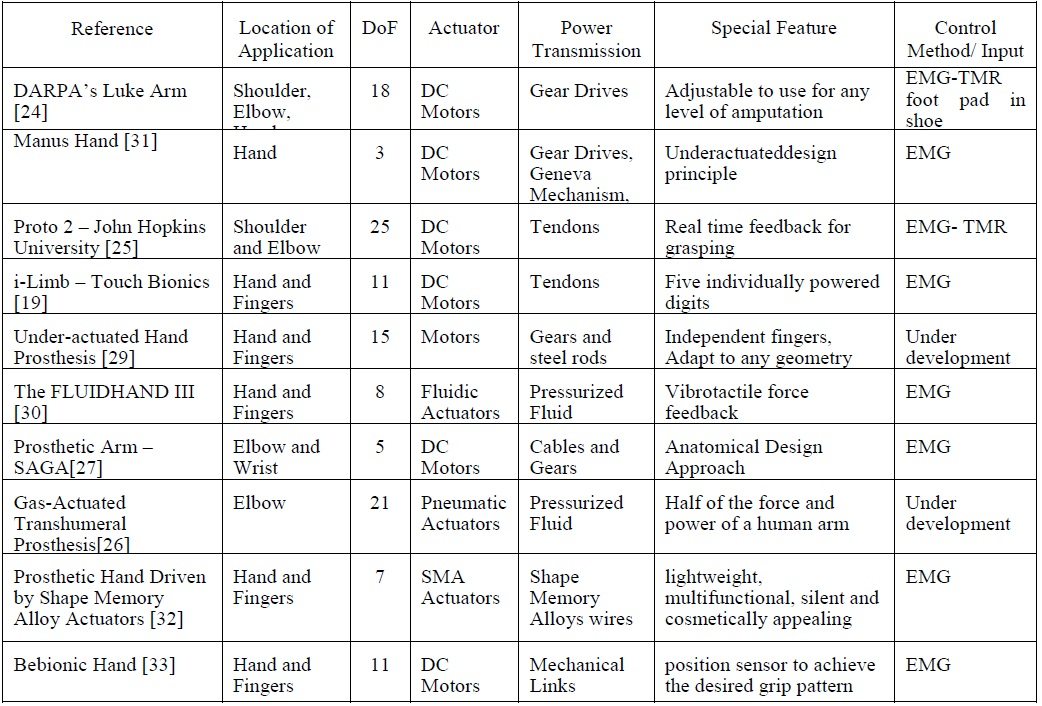
\includegraphics[width=0.7\textwidth]{graphics/hands.jpg}
			\label{graph:hand}	
			\caption{Przegląd rąk \cite{bandara2012upper}}
		\end{figure}
	\end{center}

\end{frame}


 

	\subsection{Podział}
		\begin{frame}
			\begin{center}
				\begin{figure}
					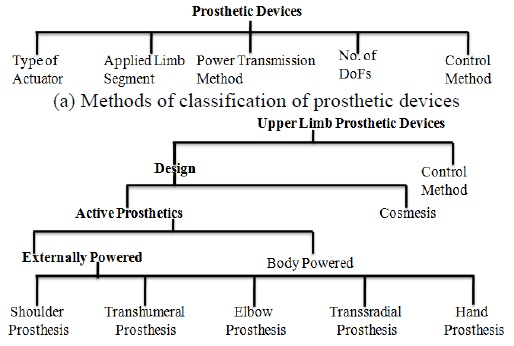
\includegraphics[width=0.7\textwidth]{graphics/classification.jpg}
					\label{graph:class}	
					\caption{Klasyfikacja \cite{bandara2012upper}}
				\end{figure}
			\end{center}
		\end{frame}							

\section{Budowa robotycznych rąk}

	\subsection{Budowa dłoni}
		\begin{frame}
			\begin{center}
				\begin{figure}
					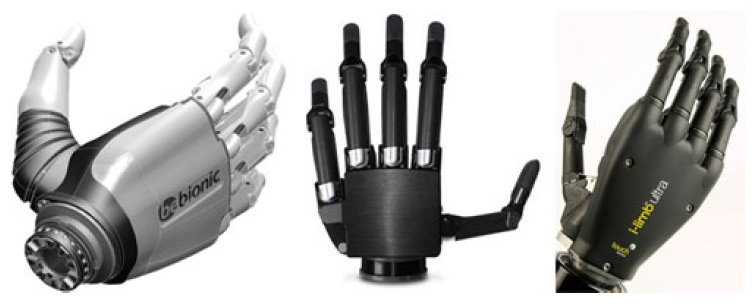
\includegraphics[width=\textwidth]{graphics/three_hand.jpg}
					\label{graph:build}	
					\caption{ \cite{6361492}}
				\end{figure}
			\end{center}
		\end{frame}				

	\subsection{Sterowanie palcem}
		\begin{frame}
			\begin{center}
				\begin{figure}
					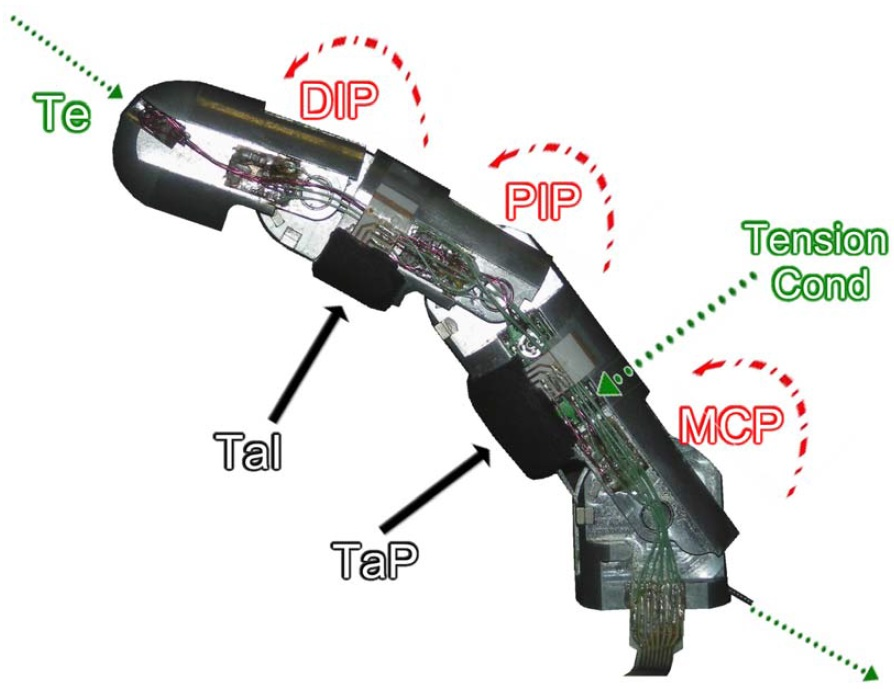
\includegraphics[width=0.7\textwidth]{graphics/smarthand_finger.jpg}
					\label{graph:build}	
					\caption{ \cite{6361492}}
				\end{figure}
			\end{center}
		\end{frame}				

		\begin{frame}
			\begin{center}
				\begin{figure}
					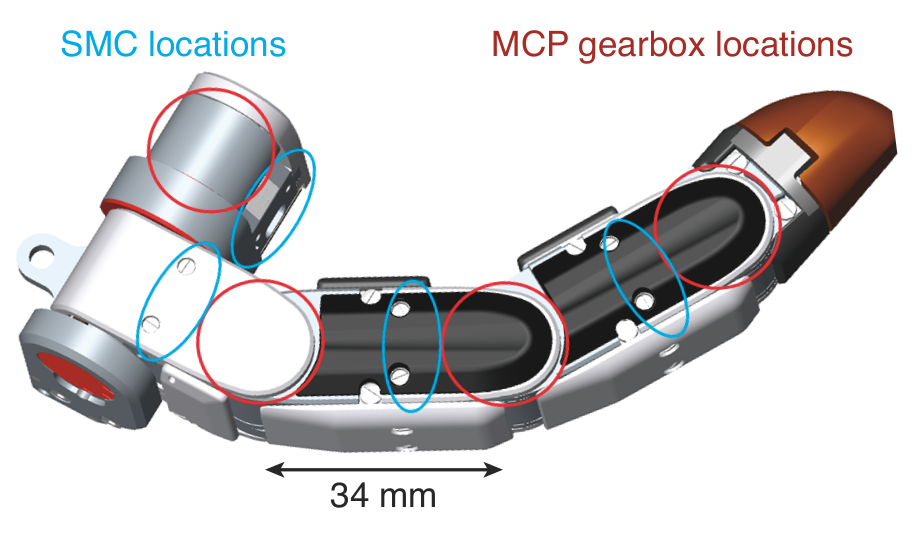
\includegraphics[width=0.7\textwidth]{graphics/finger_motors_mpl.png}
					\label{graph:build}	
					\caption{ \cite{6361492}}
				\end{figure}
			\end{center}
		\end{frame}				


\section{Ręka Bebionic}

	\begin{frame}%{Ręka Bebionic}
		bebionic3
		\begin{itemize}[<+->]
	\item osobne silniki na każdy palec, rozmieszczenie optymalnosiłowe,
	\item wydajne mikroprocesory ciągle monitorują pozycję każdego palca, dając pełną kontrolę nad protezą.
	\item 14 różnych rodzajów chwytów,
	\item adekwatna kontrola prędkości pozwala na wykonywanie precyzyjnych ruchów,
	\item możliwość przestawienia pozycji kciuka na pozycję przeciwstawną (ręczne),
	\item automatyczna kontrola siły uścisku zapobiega wyślizgiwaniu się przedmiotów,
	\item palce uginają się naturalnie przy zderzaniu się z obiektami,
	\item możliwość noszenia przedmiotów o masie do 45 kg,
		\end{itemize}

	\end{frame}

	\subsection{Podstawowa budowa}
	\begin{frame}
	\begin{center}
				\begin{figure}
					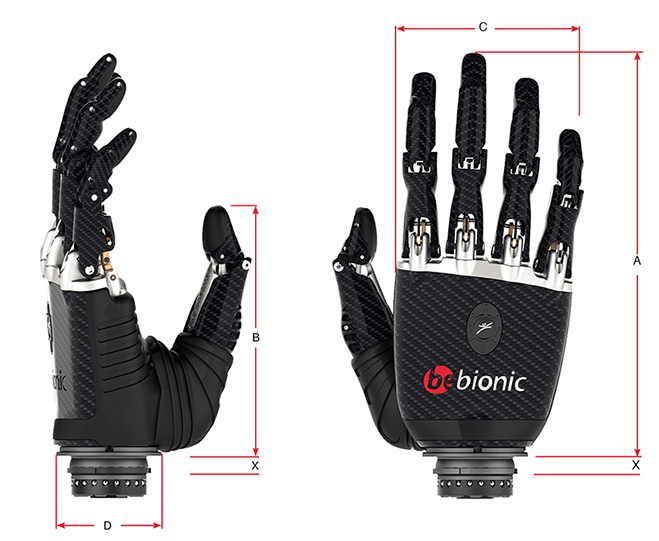
\includegraphics[width=0.7\textwidth]{graphics/bebionic_dimentions.jpg}
					\label{graph:grasp}	
					\caption{ \cite{bebionic}}
				\end{figure}
			\end{center}
	\end{frame}		
\section{Modularna kończyna}
\begin{frame}
\frametitle{Modularna kończyna}
Modularna protetyczna kończyna posiada 26 stopni swobody (ręka ludzka posiada 30). Zrobiona jest z lekkiego włókna węglowego i stopów metali o dużej wytrzymałości.
Opracowana została w projekcie DARPA (34.5mln dolarów) na Uniwersytecie Johna Hopkinsa. Jest wynikiem wielu projektów z różnych dziedzin nauki. Jej założenia to modularność, 3 rodzaje inwazyjności w ciało człowieka (pełna, częściowa, brak), lekkość, swoboda ruchu, czucie dotyknych przedmiotów.
\end{frame}
\begin{frame}
\frametitle{Modularna kończyna - widok}
\begin{figure}[htbp]
  \begin{center}
    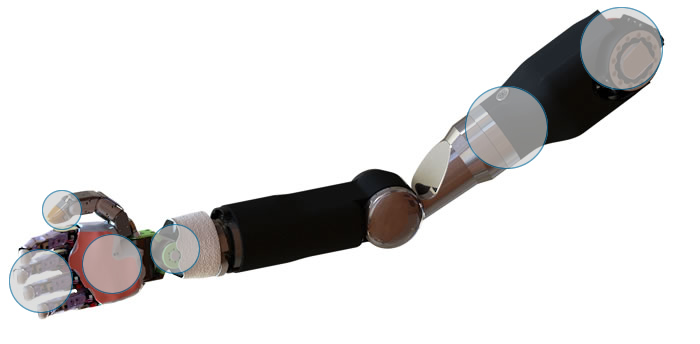
\includegraphics[width=0.9\textwidth]{graphics/arm.jpg}
  \end{center}
 \end{figure} 
\end{frame}
\subsection{Sensory}
\begin{frame}
\frametitle{Osensorowanie}
Ramię i dłoń posiadają ponad 100 czujników. Wiele technologii zostało wymyślonych i rozwiniętych specjalnie dla tej platformy. Czujniki mierzą kąt, prędkość i moment obrotowy poszczególnego stawu.
Dodatkowo czujniki na opuszkach palców mierzą:
\begin{itemize}
\item siłę przyłożoną wzdłuż 3-osi (200 Hz, 24bit res),
\item wibracje w 3-osiach (400 Hz),
\item temperaturę/strumień ciepła,
\item punkt kontaktu w 4 położeniach (400 Hz, 10 bit ADC).
\end{itemize}
\end{frame}
%---------------------------------------------------------------------------
\begin{frame}
\frametitle{Sensory - widok ręki}
\begin{figure}[htbp]
  \begin{center}
    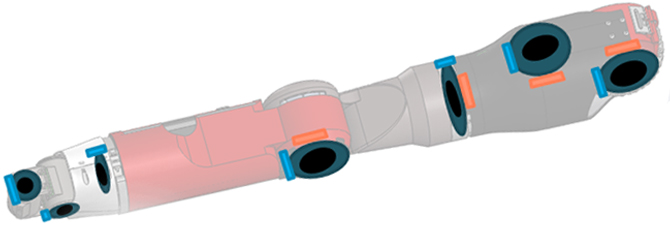
\includegraphics[width=0.9\textwidth]{graphics/arm_s.jpg}
  \end{center}
 \end{figure} 
\end{frame}
\begin{frame}
\frametitle{Sensory - widok palca}
\begin{figure}[htbp]
  \begin{center}
    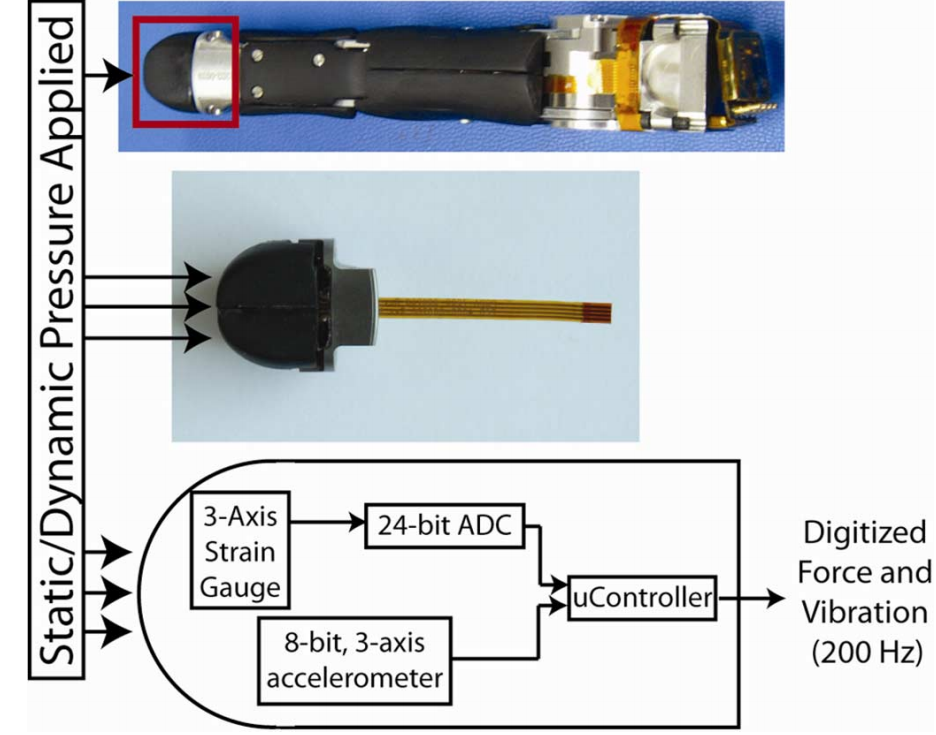
\includegraphics[width=0.7\textwidth]{graphics/Finger.png}
  \end{center}
 \end{figure} 
\end{frame}
\subsection{UEA}
%--------------------------------------------------------------------------------------------------------------------
\begin{frame}
\frametitle{UEA}
UEA (Utah Electrode Array) hybrydowa matryca zawierająca 96 elektrod o dlugści 1.5mm rozmieszczonych na kwadracie 4x4 mm.
2 matryce wszczepiane są w mózg pacjenta w ośrodek odpowiedzialny za ruch i czucie. Za wysyłanie i odbieranie danych odpowiedzilany jest
96 kanałowy dwufazowy generator pulsów (CereStim96)
\end{frame}	
\begin{frame}
\frametitle{UEA}
\begin{figure}[htbp]
  \begin{center}
    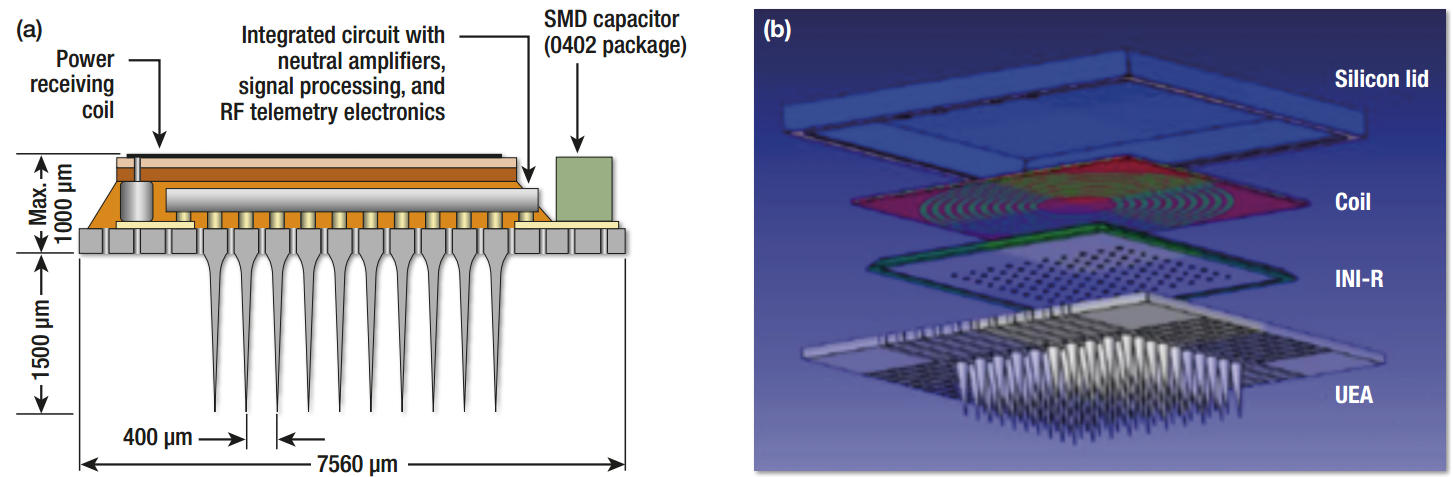
\includegraphics[width=0.9\textwidth]{graphics/UEA2.png}
  \end{center}
 \end{figure} 
\end{frame}
%--------------------------------------------------------------------------
\begin{frame}
\frametitle{UEA}
W systemie są zaprojektowane algorytmy, które przetwarzają dane sensoryczne w serie elektrycznych pobudzających impulsów, naturalnie dostrzeganych przez mózg.
\end{frame}
%--------------------------------------------------------------------------
\section{Sprzężenie zwrotne}

\begin{frame}%{Sprzężenie zwrotne}
	\begin{center}
		\begin{figure}
			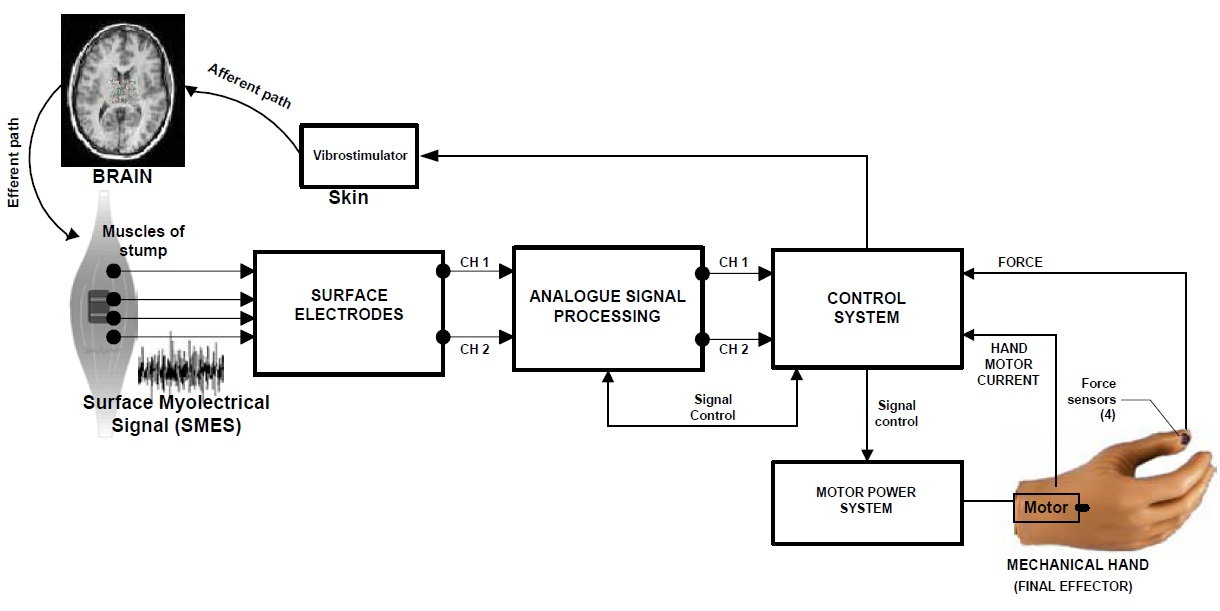
\includegraphics[width=\textwidth]{graphics/feedback.jpg}
			\label{graph:feedback}	
		\end{figure}
	\end{center}
	%\note{omówić cały obrazek}
\end{frame}


	\subsection{Pobieranie informacji}
		\begin{frame}
		Potrzebne sygnały:
			\begin{itemize}[<+->]
				\item siła uchwytu,
				\item ruch,
				\item pozycja,
				\item początek kontaktu,
				\item koniec kontaktu,
				\item dotyk, 
				\item struktura powierzchni,
				\item temperatura.
			\end{itemize}
		\end{frame}		
		
		
		
		\subsection{Przekazanie informacji od/do pacjenta}	
	
		
		\begin{frame}
			Prowadzone są badania nad trzema sposobami przesyłania informacji zwrotnej:
			\begin{itemize}[<+->]
				\item sprzężenie wibracyjne,
				\item sprzężenie elektryczne (pobudzanie skóry poprzez elektrody),
				\item sprzężenie bezpośrednio do nerwów:
				\begin{itemize}[<+->]
					\item przekazywanie informacji bezpośrednio do mózgu,
					\item przekazywanie informacji do nerwów w kikucie.
				\end{itemize}
			\end{itemize}
		\end{frame}
		
		\begin{frame}
		\begin{figure}
				\begin{center}
        			\begin{subfigure}[b]{0.5\textwidth}
                		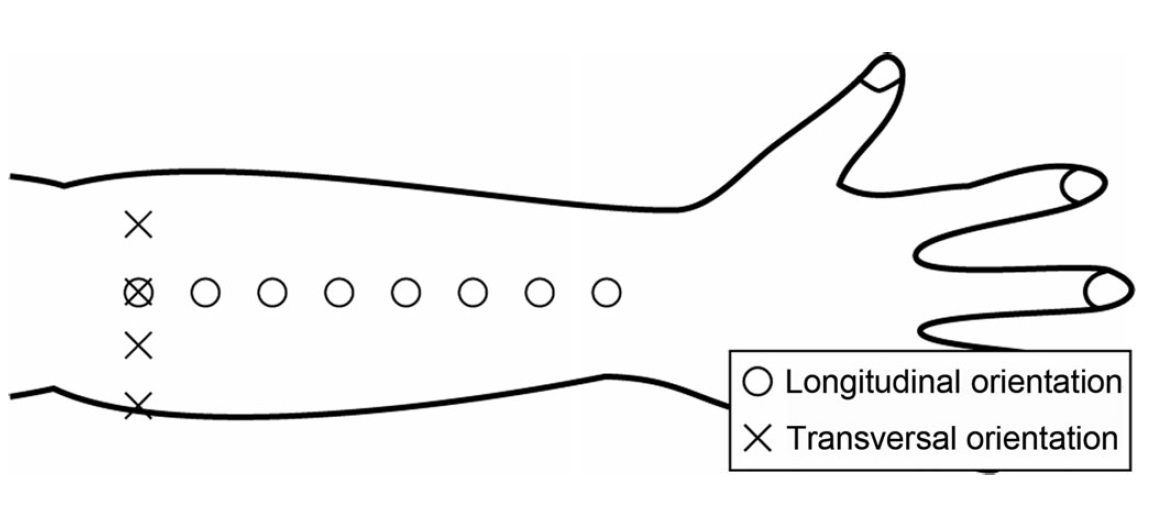
\includegraphics[width=\textwidth]{graphics/vibro_orientation.jpg}
                		\label{graph:g5}
        			\end{subfigure}%
        			\begin{subfigure}[b]{0.5\textwidth}
                		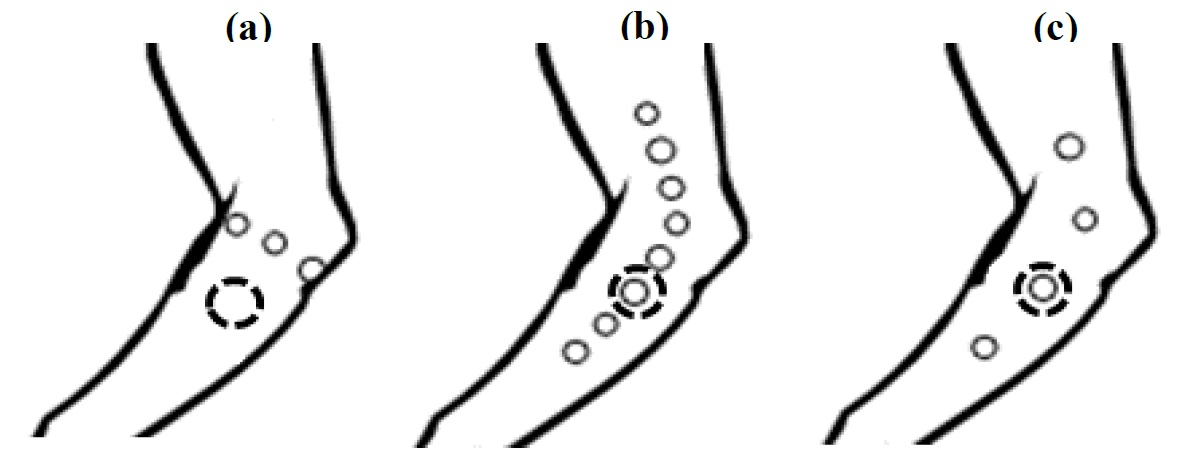
\includegraphics[width=\textwidth]{graphics/vibro_possib.jpg}
                		\label{graph:g6}
        			\end{subfigure}%
        			\newline
        			\begin{subfigure}[b]{0.7\textwidth}
                		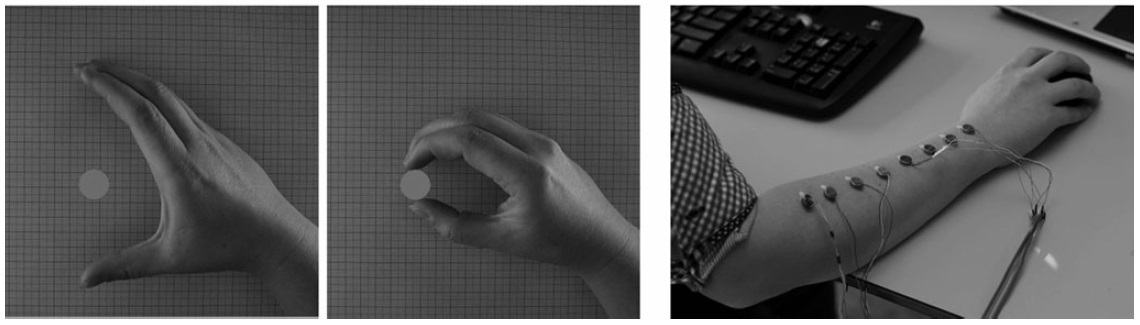
\includegraphics[width=\textwidth]{graphics/vibro_photo.jpg}
                		\label{graph:g6}
        			\end{subfigure}%
				\caption{Sprzężenie wibrostymulacyjne. \cite{tenore} }
				\end{center}
			\end{figure}
		\end{frame}
		
		\begin{frame}
		\begin{figure}
				\begin{center}
        			\begin{subfigure}[b]{0.6\textwidth}
                		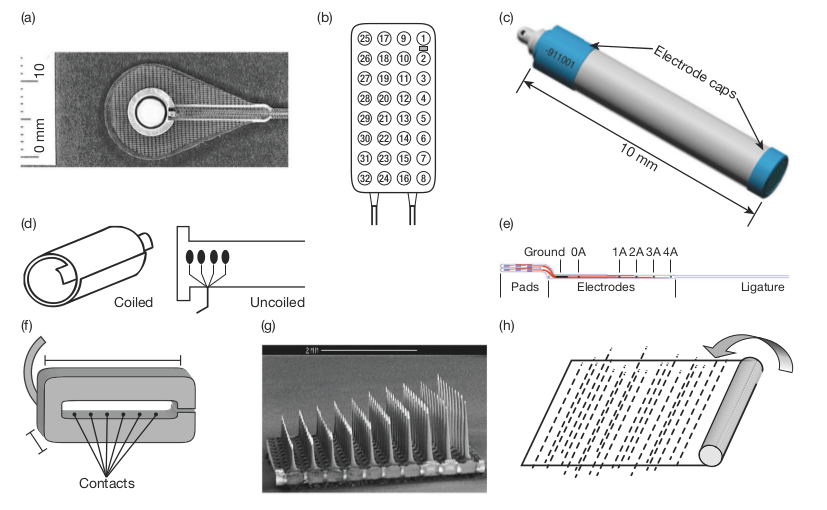
\includegraphics[width=\textwidth]{graphics/elektrode.png}
                		\label{graph:g5}
        			\end{subfigure}%
        			\begin{subfigure}[b]{0.4\textwidth}
                		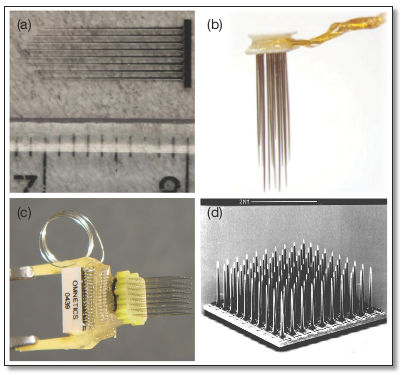
\includegraphics[width=\textwidth]{graphics/elektrode2.png}
                		\label{graph:g6}
        			\end{subfigure}%
				\caption{Mikroelektrody penetrujące. \cite{tenore} }
				\end{center}
			\end{figure}
		\end{frame}		
		
		
	\subsection{Dostępne technologie}
		\begin{frame}
			\begin{center}
				\begin{figure}
					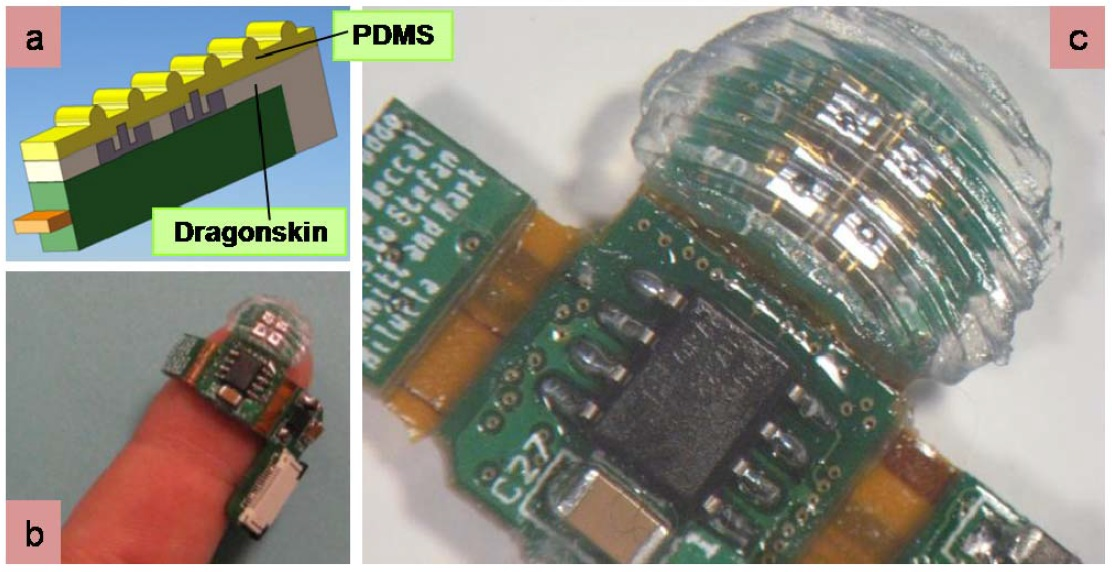
\includegraphics[width=\textwidth]{graphics/roughness_mems.jpg}
					\label{graph:mems}	
					\caption{ \cite{5420491}}
				\end{figure}
			\end{center}
		\end{frame}		
		
		
		\begin{frame}
		\begin{figure}
				\begin{center}
				
        			\begin{subfigure}[b]{0.4\textwidth}
                		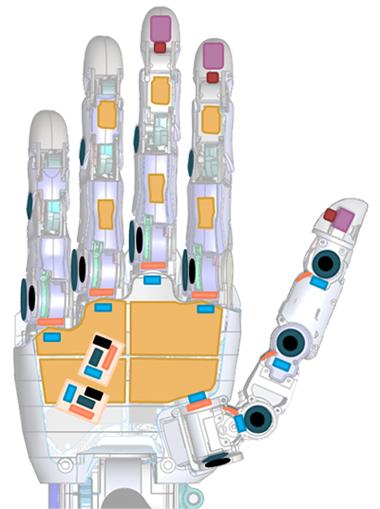
\includegraphics[width=\textwidth]{graphics/MPL_sensorhand.jpg}
                		\label{graph:g5}
        			\end{subfigure}%
        			\begin{subfigure}[b]{0.4\textwidth}
                		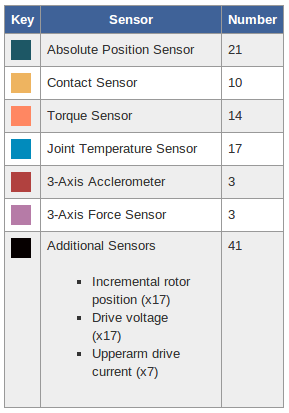
\includegraphics[width=\textwidth]{graphics/mpl_opis.png}
                		\label{graph:g6}
        			\end{subfigure}%
				\end{center}
				\caption{Sensory protezy MPL.}
			\end{figure}
		\end{frame}				
%
%		\begin{frame}
%		\begin{figure}
%				\centering
%                		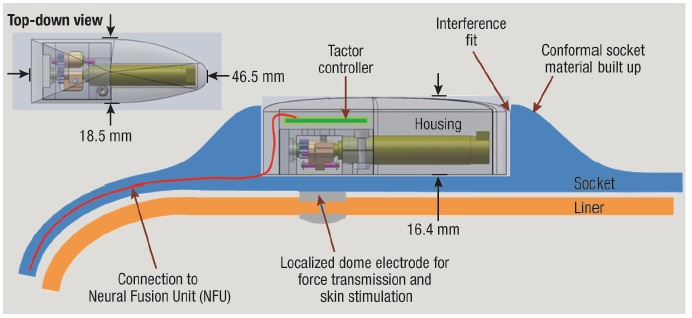
\includegraphics[width=0.7\textwidth]{graphics/vibro_mpl.jpg}
%				\caption{Wibrostymulacja dla protezy MPL.}
%			\end{figure}
%		\end{frame}	
	
		
	

\section*{Bibliografia}

\begin{frame}[allowframebreaks]
	\bibliography{bibliography}
\end{frame}
		
\begin{frame}
\begin{center}
				\begin{figure}
					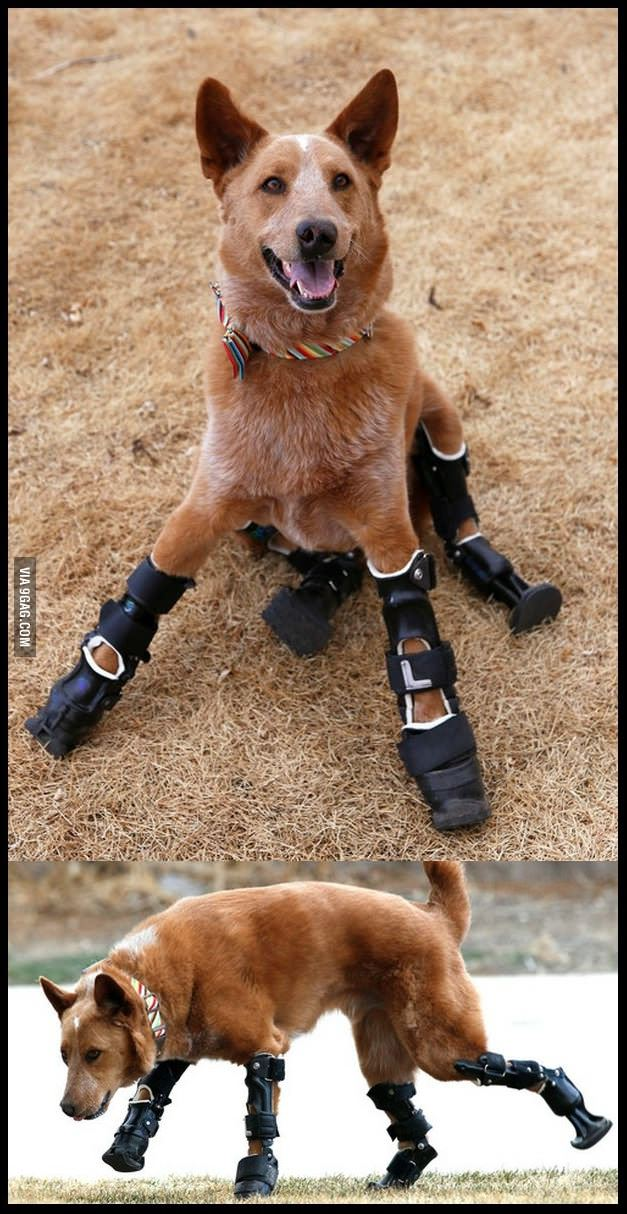
\includegraphics[width=0.3\textwidth]{graphics/dog.jpg}
					\caption{Naki’o now has 4 prosthetic legs and is able to run around happily!}
				\end{figure}
			\end{center}
\end{frame}

\end{document}
